\documentclass[11pt,a4paper]{article}
\usepackage[utf8]{inputenc}
\usepackage[T1]{fontenc}
\usepackage[brazil]{babel}
\usepackage{lmodern}
\usepackage[margin=2.5cm]{geometry}
\usepackage{amsmath,amssymb,bm}
\usepackage{booktabs,tabularx,multirow,longtable,array}
\usepackage{graphicx}
\usepackage{xcolor}
\usepackage{algorithm}
\usepackage[noend]{algpseudocode}
\usepackage[numbers,sort&compress]{natbib}
\usepackage[hidelinks]{hyperref}
\usepackage{url}
\usepackage{setspace}
\onehalfspacing

\newcommand{\todo}[1]{\textcolor{red}{[\textbf{A FAZER:} #1]}}
\newcommand{\inp}[1]{\IfFileExists{#1.tex}{\input{#1}}{\todo{tabela \texttt{\detokenize{#1}} será gerada pelos scripts de análise}}}
\newcommand{\orig}{\par\noindent\textbf{Origem.}~}
\newcommand{\func}{\par\noindent\textbf{Como funciona.}~}
\newcommand{\adap}{\par\noindent\textbf{Adaptações.}~}
\newcommand{\parm}{\par\noindent\textbf{Parâmetros.}~}
\floatname{algorithm}{Algoritmo}
\renewcommand{\algorithmicrequire}{\textbf{Entrada:}}
\renewcommand{\algorithmicensure}{\textbf{Saída:}}
\DeclareMathOperator*{\argmin}{arg\,min}
\DeclareMathOperator*{\argmax}{arg\,max}

\title{Alocação de interceptadores contra enxames de aeronaves evasivas sob informação de radar:
revisão de técnicas e avaliação comparativa reprodutível}
\author{Otávio Zordan Alves}
\date{}

\begin{document}
\maketitle

% =====================================================================================================
\begin{abstract}
Ataques com dezenas a centenas de aeronaves não tripuladas baratas, lançadas em ondas, tornaram-se frequentes na última
década e deslocaram o gargalo da defesa aérea para a \emph{decisão}: qual interceptador lançar contra qual pista de
radar, quando, e quando trocar de alvo. Essa decisão é estudada há mais de sessenta anos como atribuição arma--alvo
(WTA), mas a literatura recente se dividiu em comunidades que raramente se comparam: pesquisa operacional, robótica
multiagente, controle preditivo e aprendizado por reforço. Este artigo formula o problema como um processo de decisão
parcialmente observável, revisa as técnicas de alocação em oito famílias e \emph{implementa e compara todas elas} --- 23
algoritmos de alocação e 6 políticas aprendidas --- num mesmo simulador aberto, com relevo real, rede de radares com
difração, ruído, vieses e falsos alarmes, rastreador IMM e aeronaves que executam manobras evasivas. Um conjunto
balanceado de 60 cenários com 12 a 48 aeronaves em seis locais, dois deles reservados para teste, permite medir
desempenho, custo computacional e generalização com testes estatísticos pareados.
\todo{resumo dos resultados quantitativos quando os experimentos terminarem.}
\end{abstract}

\noindent\textbf{Palavras-chave:} atribuição arma--alvo; enxames de drones; alocação de tarefas; leilão; consenso;
metaheurísticas; aprendizado por reforço; rastreamento por radar; manobras evasivas.

\tableofcontents
\newpage

% =====================================================================================================
\section{Introdução}\label{sec:intro}

\subsection{Origem do problema}
A pergunta ``quais armas devem engajar quais alvos?'' é um dos problemas mais antigos da pesquisa operacional. Ela foi
formalizada no fim da década de 1950, no contexto da defesa contra bombardeiros e mísseis, como o problema de
\emph{atribuição arma--alvo} (\emph{weapon--target assignment}, WTA): dado um conjunto de armas, cada uma com uma
probabilidade de destruir cada alvo, e um conjunto de alvos de valores diferentes, escolher a designação que minimiza o
valor esperado dos alvos que sobrevivem~\cite{manne1958}. A primeira heurística de uso geral, o \emph{máximo retorno
marginal}, é da mesma época~\cite{denbroeder1959}. Nas décadas seguintes, a defesa contra mísseis balísticos motivou a
versão \emph{dinâmica}, em que os engajamentos ocorrem em estágios e o resultado de um estágio é observado antes do
próximo~\cite{hosein1990}, e mostrou-se que a versão geral é NP-completa~\cite{lloyd1986}. Três revisões consolidaram a
área: \citet{cai2006} sobre o WTA dinâmico, \citet{roux2007} sobre sistemas de avaliação de ameaças e atribuição de
armas (TEWA) e \citet{kline2019} sobre formulações e algoritmos exatos e heurísticos.

\subsection{O problema hoje: enxames baratos, em ondas}
Na última década, o problema mudou de escala e de natureza. Aeronaves não tripuladas baratas permitem ao atacante
lançar dezenas a centenas de vetores de uma vez, contra os quais efetores caros e escassos não são economicamente
viáveis. Alguns casos ilustram a progressão:
\begin{itemize}
  \item Em janeiro de 2018, treze pequenos drones de construção rudimentar atacaram a base aérea russa de Khmeimim e o
        ponto naval de Tartus, na Síria; segundo o relato russo, foram neutralizados por guerra eletrônica e defesa
        antiaérea~\cite{bellingcat2018}.
  \item Em setembro de 2019, o ataque às instalações de petróleo de Abqaiq e Khurais, na Arábia Saudita, combinou 18
        drones e cerca de sete mísseis de cruzeiro e interrompeu temporariamente cerca de metade da produção saudita, com
        a defesa praticamente sem engajar~\cite{idsa2019}.
  \item Em abril de 2024, o ataque iraniano contra Israel empregou mais de 300 vetores --- cerca de 170 drones, mais de 30
        mísseis de cruzeiro e mais de 120 balísticos --- e, segundo as forças israelenses, 99\,\% foram interceptados por
        uma defesa multinacional coordenada~\cite{pbs2024}.
  \item Na guerra na Ucrânia, ataques noturnos com centenas de drones do tipo Shahed levaram, a partir de 2024--2025, ao
        uso em massa de \emph{drones interceptadores} baratos, despachados contra as ameaças a partir de pistas de
        radar~\cite{pravda2025}.
\end{itemize}
O último caso é exatamente o problema deste artigo: muitos interceptadores descartáveis, cada um capaz de neutralizar uma
ameaça, despachados a partir de um quadro de radar comum contra muitas ameaças que chegam em ondas. A qualidade da
\emph{alocação} --- e não só a do sensor ou do efetor --- decide quantas ameaças passam.

\subsection{Lacunas}
Três características desse cenário ficam fora das revisões clássicas e da maior parte dos trabalhos recentes:
\begin{enumerate}
  \item \textbf{Informação imperfeita.} O decisor não vê as aeronaves, e sim pistas de radar ruidosas, sem identidade,
        limitadas pelo relevo e, muitas vezes, com mais falsos alarmes que alvos. A literatura de WTA em geral supõe alvos
        conhecidos.
  \item \textbf{Alvos evasivos.} Aeronaves que manobram, voam baixo para se esconder do radar e reagem à aproximação do
        interceptador violam a previsão de velocidade constante (ou de linha reta até o alvo) em que se apoiam quase todos
        os métodos.
  \item \textbf{Comparações incomparáveis.} Os trabalhos recentes de aprendizado por
        reforço~\cite{liu2023drones,palmas2025,jia2026}, de contra-enxame~\cite{strickland2018} e a linha brasileira do
        ITA~\cite{ricardo2023,feitosa2025,afonso2020,cruz2025} usam simuladores, métricas e linhas de base próprios, com
        poucas ameaças (de 6 a algumas dezenas) e, em geral, uma única linha de base. Não é possível saber, a partir da
        literatura, se uma política aprendida supera o método húngaro, ou se uma árvore de comportamento supera um leilão.
\end{enumerate}

\subsection{Contribuições}
\begin{itemize}
  \item Uma \textbf{formulação} do problema como processo de decisão de Markov parcialmente observável, decomposta em
        avaliação de ameaças, alocação e guiagem, que explicita o que cada família de métodos supõe sobre a informação e
        sobre o alvo (Seção~\ref{sec:problema}).
  \item Uma \textbf{revisão} das técnicas de alocação em oito famílias, da pesquisa operacional ao aprendizado por
        reforço, com uma comparação estruturada dos trabalhos mais próximos (Seção~\ref{sec:revisao}).
  \item A \textbf{implementação de todas as técnicas revisadas} numa interface comum --- 29 métodos, cada um descrito por
        origem, funcionamento, adaptações e parâmetros ---, com a verificação de que as implementações reproduzem as
        equivalências teóricas conhecidas (Seção~\ref{sec:metodos}).
  \item Uma \textbf{avaliação reprodutível} num simulador aberto e num conjunto balanceado de 60 cenários com até 48
        aeronaves evasivas, com divisão treino/teste por local, sementes pareadas e testes estatísticos
        (Seções~\ref{sec:ambiente}--\ref{sec:resultados}).
\end{itemize}

% =====================================================================================================
\section{Formulação do problema}\label{sec:problema}

\subsection{Cenário}
Uma região contém zonas prioritárias $\mathcal{Z}$ (círculos que representam ativos a defender) e bases de
interceptadores. Um conjunto $\mathcal{A}$ de $N$ aeronaves entra na região em ondas e segue rotas que terminam num
ponto de impacto. Uma aeronave que chega ao impacto sem ser interceptada causa dano $w_a=w_P=10$ se o impacto é numa zona
prioritária e $w_a=w_O=1$ fora. Há $M\ge N$ interceptadores descartáveis distribuídos pelas bases, cada um com
velocidade $v_d$, autonomia $T_d$ e um sensor próprio de alcance $r_s$; um interceptador neutraliza uma aeronave por
contato a menos de $r_c$ e é consumido. A Tabela~\ref{tab:notacao} resume a notação.

\begin{table}[t]
\centering
\caption{Notação principal.}
\label{tab:notacao}
\small
\begin{tabularx}{\textwidth}{@{}lX@{}}
\toprule
Símbolo & Significado \\
\midrule
$\mathcal{A}$, $N$; $\mathcal{D}$, $M$ & aeronaves e seu número; interceptadores e seu número \\
$w_a$; $w_P=10$, $w_O=1$ & dano da aeronave $a$; dano dentro e fora de zona prioritária \\
$v_d$, $T_d$, $r_s$, $r_c$ & velocidade, autonomia, alcance do sensor e raio de contato do interceptador \\
$\mathcal{P}(t)=\{p_j\}$ & quadro de radar: pistas com posição $\bm{x}_j$, velocidade $\bm{v}_j$, incerteza, idade \\
$\mathcal{D}_t$ & fila de interceptadores que decidem na rodada $t$ \\
$x_{ij}\in\{0,1\}$ & designação do interceptador $i$ à pista $j$ \\
$t^\star_{ij}$, $c_{ij}$ & tempo previsto de interceptação; custo com histerese (E2) \\
$w_j$, $t^Z_j$ & peso de prioridade e tempo até a zona inferidos da pista (E3) \\
$q_{ij}$, $V_j$, $S_j$ & probabilidade de sucesso, valor e sobrevivência da pista (E4) \\
$F(\bm{x})$ & valor esperado destruído numa rodada \eqref{eq:F} \\
$D$ & dano normalizado de um episódio \eqref{eq:dano} \\
\bottomrule
\end{tabularx}
\end{table}

\subsection{Formulação como processo de decisão parcialmente observável}
O problema é um processo de decisão de Markov parcialmente observável (POMDP) em tempo discreto, com rodadas de
decisão a cada $\Delta_d$:
\begin{itemize}
  \item \textbf{Estado} $s_t$: posição, velocidade, rota, perfil de manobra e situação (viva, interceptada, caída) de cada
        aeronave; posição, autonomia, alvo e situação (na base, em voo, consumido) de cada interceptador; estado interno
        do rastreador.
  \item \textbf{Observação} $o_t$: o quadro de radar $\mathcal{P}(t)$ (pistas sem identidade, com falsos alarmes e sem as
        aeronaves fora de cobertura), o estado dos próprios interceptadores e as zonas prioritárias. A rota, o ponto de
        impacto, o perfil de manobra e a legitimidade das pistas não são observados.
  \item \textbf{Ação} $a_t$: para cada interceptador da fila $\mathcal{D}_t$ (os ociosos nas bases e os em voo cuja
        reavaliação venceu), uma pista de $\mathcal{P}(t)$ ou a ação nula (esperar ou manter o alvo), isto é, uma matriz
        $\bm{x}\in\{0,1\}^{|\mathcal{D}_t|\times|\mathcal{P}(t)|}$ com
        \begin{equation}
          \sum_j x_{ij}\le1\quad\forall i,\qquad \sum_i x_{ij}+n_j^0\le\bar n\quad\forall j,
          \label{eq:restr}
        \end{equation}
        em que $n_j^0$ interceptadores já perseguem a pista $j$ e $\bar n$ é o limite por pista (1 por padrão).
  \item \textbf{Transição}: as aeronaves avançam pelas rotas com manobras evasivas; os interceptadores em trânsito voam
        para o ponto previsto de encontro da sua pista e, no alcance do sensor, passam à guiagem terminal; o radar mede e o
        rastreador atualiza as pistas. Há contato quando a distância de passagem é menor que $r_c$, e impacto quando uma
        aeronave chega ao fim da rota.
  \item \textbf{Objetivo}: minimizar o dano normalizado esperado,
        \begin{equation}
          \min_{\pi}\ \mathbb{E}_\pi[D],\qquad
          D = \frac{\sum_{a\in\mathcal{A}} w_a\,\mathbf{1}\{a\text{ atinge o impacto}\}}{\sum_{a\in\mathcal{A}} w_a}\in[0,1],
          \label{eq:dano}
        \end{equation}
        sobre políticas $\pi$ que mapeiam o histórico de observações em ações.
\end{itemize}
Resolver esse POMDP exatamente é inviável: o espaço de ações é combinatório (atribuições entre dezenas de
interceptadores e pistas), o estado é contínuo e de alta dimensão, e o comportamento evasivo do alvo não é conhecido.
Todos os métodos práticos decompõem o problema e aproximam a política.

\subsection{Decomposição em camadas}
A decisão se decompõe em três camadas, que correspondem às famílias de métodos da literatura:
\begin{enumerate}
  \item \textbf{Avaliação de ameaças}: quais pistas são aeronaves reais, quão perigosas são e quanto tempo há até o dano.
  \item \textbf{Alocação}: dada a avaliação, qual interceptador vai contra qual pista nesta rodada, e quais esperam.
  \item \textbf{Guiagem}: dado o alvo, como o interceptador o alcança.
\end{enumerate}
Este artigo compara técnicas da camada de \emph{alocação}, com as outras duas fixas: a avaliação de ameaças é uma regra
física comum (E1) ou um classificador aprendido, e a guiagem é uma lei fixa, escolhida por um experimento separado
(Seção~\ref{sec:res_guiagem}).

\subsection{Relação com o WTA}
Restrita a uma rodada, a alocação é uma instância do WTA estático~\cite{manne1958}: designar armas $i$ a alvos $j$ de
valor $V_j$, com probabilidade de abate $q_{ij}$, minimizando o valor sobrevivente esperado,
\begin{equation}
  \min_{x}\ \sum_{j} V_j \prod_{i} (1-q_{ij})^{x_{ij}}\quad\text{s.a. \eqref{eq:restr}}.
  \label{eq:wta}
\end{equation}
O nosso problema difere do WTA clássico em três pontos: é \emph{dinâmico} (a alocação se repete e pode ser revista, como
no WTA dinâmico~\cite{hosein1990}), \emph{parcialmente observável} (alocam-se pistas, que podem ser falsas, e não alvos) e
\emph{acoplado à cinemática} ($q_{ij}$ não é dado, depende do tempo de interceptação e da manobra do alvo). Com no máximo
um interceptador por pista e $q_{ij}\approx1$, \eqref{eq:wta} se reduz ao problema de atribuição linear~\cite{kuhn1955}.

\subsection{Elementos comuns a todos os métodos}\label{sec:comuns}
Quatro grandezas, calculadas só a partir das observações, são usadas por quase todos os métodos.

\paragraph{(E1) Filtro de plausibilidade.} Para não gastar interceptadores com falsos alarmes, os métodos só consideram
pistas dentro do envelope de voo de uma aeronave:
\begin{equation}
  \Pi(p_j)=\mathbf{1}\{15\le\|\bm{v}_{j}^{h}\|\le42\}\,\mathbf{1}\{|v_{j}^{z}|\le8\}\,\mathbf{1}\{-20\le h_j^{\mathrm{AGL}}\le500\}
  \label{eq:plaus}
\end{equation}
(velocidades em m/s, altura sobre o terreno em m). É a forma mais simples de avaliação de ameaças; as redes neurais a
trocam por um classificador aprendido.

\paragraph{(E2) Custo de interceptação.} O tempo $t^\star_{ij}$ que o interceptador $i$ leva até o ponto previsto de
encontro com a pista $j$, supondo que ela mantém a velocidade estimada, é a menor raiz positiva de
\begin{equation}
  (\|\bm{v}_j\|^2-v_d^2)\,t^2+2\,(\bm{r}_{ij}\!\cdot\!\bm{v}_j)\,t+\|\bm{r}_{ij}\|^2=0,\qquad \bm{r}_{ij}=\bm{x}_j-\bm{x}_i .
  \label{eq:tint}
\end{equation}
O custo usado pelos métodos é
\begin{equation}
  c_{ij} = \begin{cases} \kappa^{\mathbf{1}\{j=j_i\}}\,t^\star_{ij}, & t^\star_{ij}\le T_d-\tau_i,\\ \infty, & \text{caso contrário,}\end{cases}
  \label{eq:custo}
\end{equation}
em que $\tau_i$ é o tempo já voado e $j_i$ a pista atual. A \emph{histerese} $\kappa=0{,}7$ faz o interceptador só trocar
de alvo se a alternativa for 30\,\% mais rápida; sem ela, pistas ruidosas o fazem oscilar. Como~\eqref{eq:tint} supõe
velocidade constante, as manobras evasivas aparecem como erro nesse custo.

\paragraph{(E3) Peso de prioridade e tempo até a zona.} O ponto de impacto não é observado; a prioridade é inferida pela
geometria. Com $d_j$ a distância assinada da pista à zona prioritária mais próxima (negativa dentro) e $\dot d_j$ a sua
velocidade de aproximação,
\begin{equation}
  w_j=\begin{cases} w_P, & d_j\le 0,\\ (w_P+w_O)/2, & \dot d_j>5\text{ m/s e } d_j<3\text{ km},\\ w_O, & \text{caso contrário;}\end{cases}
  \qquad
  t^Z_j=\begin{cases}0, & d_j\le0,\\ d_j/\dot d_j, & \dot d_j>1,\\ \infty,&\text{caso contrário.}\end{cases}
  \label{eq:peso}
\end{equation}
As fintas do conjunto de cenários foram desenhadas para enganar exatamente essa inferência.

\paragraph{(E4) Modelo de sucesso e objetivo WTA.} Os métodos derivados do WTA precisam de $q_{ij}$, que estimamos por
\begin{equation}
  q_{ij} = P_T\,e^{-c_{ij}/\tau_q}\,\mathbf{1}\{c_{ij}<\infty\},\qquad P_T=0{,}85,\ \tau_q=600\text{ s},
  \label{eq:q}
\end{equation}
com $P_T$ calibrado pelo experimento de guiagem (Seção~\ref{sec:res_guiagem}) e o decaimento representando a perda de
chance em trânsitos longos. Com valor $V_j=w_j$ e sobrevivência $S_j=\prod_{k\in\mathcal{F}_j}(1-q_{kj})$ dada pelos
interceptadores $\mathcal{F}_j$ já em voo contra $j$, o objetivo de uma rodada é o valor esperado destruído,
\begin{equation}
  F(\bm{x}) = \sum_j V_j S_j\Big[1-\prod_{i}(1-q_{ij})^{x_{ij}}\Big]
  - \sum_{i}\ell_i\sum_j x_{ij}
  - M\sum_j\max\!\Big(0,\ n_j^0+\sum_i x_{ij}-\bar n\Big),
  \label{eq:F}
\end{equation}
que é~\eqref{eq:wta} como maximização. O custo de lançamento $\ell_i=0{,}05$ (só para interceptadores na base) impede o
ótimo trivial de lançar tudo de uma vez e preserva interceptadores para as ondas seguintes; o último termo ($M=10$) impõe
o limite~\eqref{eq:restr} como penalidade.

% =====================================================================================================
\section{Revisão da literatura}\label{sec:revisao}

Organizamos as técnicas de alocação em oito famílias. Para cada uma, descrevemos a ideia central, a evolução e os
resultados principais, e a hipótese sobre informação e alvo. A Tabela~\ref{tab:relacionados} compara os trabalhos mais
próximos do nosso.

\subsection{Regras gulosas e TEWA}
Os sistemas de avaliação de ameaças e atribuição de armas (TEWA) separam a decisão em duas etapas: avaliar cada ameaça
--- pelo tempo até o ativo defendido, pela distância do ponto de maior aproximação e pela capacidade inferida --- e
designar efetores na ordem de ameaça~\cite{roux2007}. A revisão de \citet{roux2007} e a avaliação de sistemas TEWA de
\citet{johansson2010} mostram que, na prática, predominam regras simples e transparentes: designar o efetor que alcança
a ameaça mais cedo, ou atender primeiro a ameaça mais urgente. Essas regras são rápidas e auditáveis, mas míopes: decidem
uma ameaça ou um efetor de cada vez e dependem da ordem em que o fazem. Todas preveem o alvo com velocidade constante.

\subsection{Atribuição ótima}
Quando cada alvo recebe no máximo um efetor e o custo de um par não depende dos demais, a alocação de uma rodada é um
problema de atribuição linear. O método húngaro~\cite{kuhn1955,munkres1957} o resolve exatamente em tempo polinomial,
o que o torna a linha de base natural para métodos aprendidos~\cite{liu2023drones}. O algoritmo de leilão de
Bertsekas~\cite{bertsekas1988} resolve o mesmo problema por um mecanismo de preços em que cada agente só usa informação
local, e por isso é a ponte entre a atribuição ótima e a alocação distribuída. A limitação comum é a miopia temporal: a
solução é ótima para a rodada, não para o episódio.

\subsection{WTA e retorno marginal}
O WTA com probabilidades de abate~\eqref{eq:wta} é não linear e NP-completo~\cite{lloyd1986}. O máximo retorno marginal
(MMR)~\cite{denbroeder1959} constrói a solução inserindo, a cada passo, o par arma--alvo que mais reduz o valor
sobrevivente; é ótimo para armas idênticas e é o ponto de partida da maioria das heurísticas. \citet{ahuja2007}
apresentaram limitantes por programação linear, inteira e fluxo em rede para \emph{branch-and-bound}, resolvendo à
otimalidade instâncias de até $80\times80$, e uma busca em vizinhança de grande escala (VLSN) que chega perto do ótimo
em instâncias de $200\times200$ em segundos. \citet{kline2019} revisam essas e outras abordagens exatas e heurísticas. A
literatura de WTA em geral supõe que os alvos e as probabilidades de abate são conhecidos.

\subsection{Metaheurísticas}
Algoritmos genéticos~\cite{lee2003ga}, colônias de formigas~\cite{lee2002aco}, enxame de partículas e recozimento
simulado formam a família mais numerosa na literatura de WTA~\cite{kline2019}. Tratam objetivos e restrições arbitrários
e foram aplicados a variantes com múltiplos tipos de armas e restrições operacionais. \citet{lee2003ga} mostraram a
importância de semear a população com soluções gulosas (``eugenia gulosa''), e \citet{lee2002aco} combinaram colônia de
formigas com mecanismos imunológicos. As limitações são a ausência de garantias e um tempo de execução difícil de limitar
em tempo real; num problema dinâmico, cada rodada exige uma nova otimização.

\subsection{Alocação distribuída}
Na robótica multiagente, \citet{gerkey2004} classificaram a alocação de tarefas pelo número de tarefas por robô, de
robôs por tarefa e pelo horizonte de planejamento; interceptadores descartáveis são o caso ``uma tarefa por robô, um robô
por tarefa, atribuição instantânea''. O CBAA e o CBBA~\cite{choi2009} combinam lances locais com consenso sobre os
vencedores e convergem para atribuições sem conflito, com garantia de 50\,\% do ótimo, mesmo com consciência situacional
inconsistente entre os agentes. São a referência para enxames sem decisor central. No regime de uma tarefa por agente
com comunicação completa, o CBAA equivale ao guloso global.

\subsection{Alocação dinâmica}
No WTA dinâmico~\cite{hosein1990,cai2006}, os engajamentos se repetem em estágios e o resultado de cada um é observado
antes do próximo. Dessa literatura vêm duas lições usadas aqui: vale reservar efetores quando as ameaças chegam em ondas,
e o esquema \emph{shoot--look--shoot} --- observar o resultado antes de engajar de novo --- economiza efetores em relação a
salvas. Políticas de horizonte deslizante, que resolvem a cada estágio um problema estático com o estado atual, são a
aproximação prática do ótimo dinâmico, e é assim que todos os métodos conjuntos deste trabalho operam.

\subsection{Alocação integrada à trajetória}
Uma alternativa a separar alocação e guiagem é resolvê-las juntas por otimização. \citet{afonso2020} formulam alocação
de tarefas e planejamento de trajetória de múltiplos agentes, com obstáculos e restrições de conectividade, como um
programa linear inteiro misto (MILP) de horizonte deslizante. \citet{cruz2025} leva a ideia à neutralização de ameaças
aéreas com um MIQP tridimensional que inclui limites de velocidade e aceleração, obstáculos, bateria na métrica de
alocação e alinhamento da velocidade terminal com a do alvo, validado em realidade mista com três drones reais. Essa
família produz trajetórias viáveis e alocações ótimas para o modelo previsto, mas o número de variáveis binárias cresce
com agentes $\times$ alvos $\times$ passos do horizonte, a previsão do alvo é de velocidade constante, e o próprio autor
aponta o tempo de solução como o limitante para operação em malha fechada.

\subsection{Arquiteturas comportamentais}
Árvores de comportamento, originárias dos jogos digitais, codificam a política de cada agente numa hierarquia legível de
condições e ações e se difundiram na robótica pela modularidade. \citet{ricardo2023} as aplicam à proteção de um drone
líder contra ameaças kamikaze, com alocação por distância numa arquitetura líder--seguidor e um simulador físico.
\citet{feitosa2025} tornam a decisão descentralizada e baseada em utilidade: cada defensor avança sobre uma ameaça quando
uma função afim do tempo de deslocamento, da ameaça do alvo e da ameaça composta é positiva, com coeficientes ajustados
por algoritmo genético; com 3 defensores contra 6 ameaças em linha reta e consciência situacional completa, a defesa
resiste a cenários de dificuldade crescente. Num contexto relacionado, \citet{strickland2018} discutem táticas de
contra-enxame contra ataques de saturação, de estratégias de perseguição--evasão a modelos de atrito de Lanchester.

\subsection{Aprendizado}
Os métodos aprendidos têm três vertentes. Na \emph{imitação}, uma rede reproduz um especialista --- tipicamente um
algoritmo ótimo, porém mais lento --- e o DAgger~\cite{ross2011} corrige o acúmulo de erros nos estados que a própria rede
visita. No \emph{reforço com política centralizada}, uma rede escolhe a ação a partir do conjunto de alvos; como esse
número varia, usam-se arquiteturas invariantes à ordem, por agregação (DeepSets~\cite{zaheer2017}) ou por
atenção~\cite{vaswani2017}, que \citet{kool2019} mostraram eficazes em problemas combinatórios. \citet{liu2023drones}
treinam uma política de reforço para alocação em enxames e relatam vantagens sobre o húngaro em tolerância a falhas e
tempo de execução; \citet{palmas2025} treina uma política de priorização de interceptações e relata menos dano que uma
regra manual. No \emph{reforço multiagente}, \citet{jia2026} combinam atenção em grafos para a alocação com MAPPO para a
manobra, em escalas de tempo separadas. Em todos, a comparação é com uma ou duas linhas de base, em simulador próprio.

\subsection{Guiagem e rastreamento}
A eficácia de uma designação depende de componentes fora da alocação: a guiagem terminal (perseguição pura, navegação
proporcional e variantes~\cite{shneydor1998,zarchan2012,palumbo2010}, inclusive para drones~\cite{pliska2024}) e a
qualidade das pistas (rastreamento IMM~\cite{blom1988}, associação de dados~\cite{barshalom2001}, detecção de alvos
flutuantes~\cite{swerling1960}). Neste trabalho, ambos são componentes fixos do ambiente.

\begin{table}[t]
\centering
\caption{Comparação dos trabalhos mais próximos. Escala: defensores $\times$ ameaças. Informação: o que o decisor
observa. Alvo: modelo de movimento das ameaças.}
\label{tab:relacionados}
\scriptsize
\renewcommand{\arraystretch}{1.25}
\begin{tabularx}{\textwidth}{@{}>{\raggedright}p{2.2cm}>{\raggedright}p{2.6cm}>{\raggedright}p{1.6cm}>{\raggedright}p{2.2cm}>{\raggedright}p{2.0cm}>{\raggedright\arraybackslash}X@{}}
\toprule
Trabalho & Método & Escala & Informação & Alvo & Comparação \\
\midrule
Ricardo Jr et al.~\cite{ricardo2023} & árvore, alocação por distância & poucos & completa & kamikaze em linha reta & simulador físico próprio \\
Feitosa et al.~\cite{feitosa2025} & árvore com utilidade, GA & $3\times6$ & completa (radar central) & linha reta & 9 cenários, sem linha de base \\
Afonso et al.~\cite{afonso2020} & MILP de horizonte deslizante & poucos & completa & tarefas fixas & cenários de demonstração \\
Cruz~\cite{cruz2025} & MIQP de horizonte deslizante & $3\times3$ & posição e velocidade por radar & velocidade constante & simulação e realidade mista \\
Liu et al.~\cite{liu2023drones} & reforço profundo & enxame & completa & -- & húngaro \\
Palmas~\cite{palmas2025} & reforço profundo & configurável & ruidosa e parcial & rotas pré-definidas & regra manual \\
Jia et al.~\cite{jia2026} & atenção em grafos + MAPPO & enxame & -- & intrusão dinâmica & linhas de base de reforço \\
\midrule
Este trabalho & 29 métodos de 8 famílias & até $60\times48$ & radar com falsos alarmes, relevo e vieses & 5 perfis evasivos & todos contra todos, testes pareados \\
\bottomrule
\end{tabularx}
\end{table}

% =====================================================================================================
\section{Métodos implementados}\label{sec:metodos}

\subsection{Catálogo}
A Tabela~\ref{tab:catalogo} lista os 29 métodos implementados, numerados de M1 a M29, com a origem, o funcionamento e
a adaptação de cada um em uma linha. As subseções seguintes detalham cada família com o mesmo roteiro: \textbf{origem},
\textbf{como funciona}, \textbf{adaptações} e \textbf{parâmetros}.

Todos usam a mesma interface. A cada rodada, recebem o quadro de pistas e as zonas prioritárias e devolvem uma ação
para cada interceptador da fila. Os métodos \emph{individuais} (gulosos e árvores) decidem um interceptador por vez, na
ordem da fila; os \emph{conjuntos} resolvem a rodada inteira (todos os interceptadores da fila contra todas as pistas) e
entregam a cada um a sua parte. Nenhum método acessa a posição verdadeira das aeronaves nem o rótulo de legitimidade das
pistas. Exceto M1 e M8, todos aplicam o filtro (E1).

\begin{table}[p]
\centering
\caption{Catálogo dos métodos implementados. \emph{Ind.}: decide um interceptador por vez; \emph{conj.}: resolve a rodada
inteira. As referências são as de origem; a coluna de adaptação resume o que mudou para o nosso problema.}
\label{tab:catalogo}
\scriptsize
\renewcommand{\arraystretch}{1.25}
\begin{tabularx}{\textwidth}{@{}l>{\raggedright}p{2.6cm}>{\raggedright}p{1.6cm}>{\raggedright\arraybackslash}X>{\raggedright\arraybackslash}X@{}}
\toprule
\# & Método & Origem & Como funciona & Adaptação \\
\midrule
\multicolumn{5}{@{}l}{\emph{Regras simples}} \\
M1 & Aleatório & -- & pista sorteada, sem filtro, nunca troca (ind.) & piso de desempenho \\
M2 & Guloso (próximo) & \cite{kline2019} & menor $c_{ij}$ (ind.) & -- \\
M3 & Guloso (urgente) & \cite{kline2019} & menor folga até o solo (ind.) & folga estimada só pelo radar \\
M4 & Guloso (prioridade) & \cite{kline2019} & menor $c_{ij}/w_j$ (ind.) & peso inferido pela geometria (E3) \\
M5 & TEWA sequencial & \cite{roux2007} & ordena por ameaça, designa o mais rápido (conj.) & ameaça = peso / tempo até a zona \\
\midrule
\multicolumn{5}{@{}l}{\emph{Atribuição ótima (um interceptador por pista)}} \\
M6 & Húngaro & \cite{kuhn1955,munkres1957} & atribuição de mínimo tempo total (conj.) & custo com histerese (E2) \\
M7 & Húngaro ponderado & \cite{kuhn1955} & idem, tempo dividido pelo peso (conj.) & especialista das redes \\
M8 & Húngaro pond. sem filtro & \cite{kuhn1955} & M7 sem o filtro (E1) & mede o valor do filtro \\
M9 & Leilão & \cite{bertsekas1988} & lances e preços até o equilíbrio (conj.) & versão assimétrica sem escalonamento de $\varepsilon$ \\
\midrule
\multicolumn{5}{@{}l}{\emph{Alocação distribuída}} \\
M10 & Guloso global & \cite{choi2009} & fixa o par de maior lance, repete (conj.) & forma centralizada do CBAA \\
M11 & CBAA & \cite{choi2009} & lances locais + consenso de máximo (conj.) & comunicação completa via estação central \\
M12 & CBAA com comunic. local & \cite{choi2009} & idem, grafo de 3~km, 3 rodadas & conflitos resolvidos por ordem de chegada \\
\midrule
\multicolumn{5}{@{}l}{\emph{WTA (objetivo de valor esperado \eqref{eq:F})}} \\
M13 & MMR & \cite{denbroeder1959} & insere o par de maior ganho marginal (conj.) & custo de lançamento decide esperar \\
M14 & Húngaro sobre WTA & \cite{ahuja2007} & solução exata de \eqref{eq:F} com $\bar n=1$ (conj.) & coluna ``esperar'' por interceptador \\
M15 & MILP (HiGHS) & \cite{afonso2020,cruz2025} & mesmo problema como programa inteiro & parte de alocação do MPC inteiro \\
M16 & Busca local (VLSN) & \cite{ahuja2007} & melhora o MMR por realocação e troca & vizinhança polinomial \\
\midrule
\multicolumn{5}{@{}l}{\emph{Metaheurísticas (objetivo \eqref{eq:F}, semeadas com o MMR)}} \\
M17 & Algoritmo genético & \cite{lee2003ga} & torneio, cruzamento uniforme, mutação, elitismo & semente gulosa (``eugenia'') \\
M18 & Colônia de formigas & \cite{lee2002aco} & construção probabilística guiada por feromônio & opção ``esperar'' como caminho \\
M19 & Recozimento simulado & \cite{kline2019} & aceita pioras com prob. decrescente & parte do MMR \\
M20 & Enxame de partículas & \cite{kline2019} & partículas contínuas decodificadas por chave & codificação por chaves aleatórias \\
\midrule
\multicolumn{5}{@{}l}{\emph{Alocação dinâmica}} \\
M21 & Húngaro com reserva & \cite{hosein1990} & M7, mas guarda 20\,\% dos interceptadores & reserva só usada por pistas prioritárias \\
\midrule
\multicolumn{5}{@{}l}{\emph{Arquiteturas comportamentais}} \\
M22 & Árvore (distância) & \cite{ricardo2023} & engaja a mais próxima a menos de 4~km (ind.) & sem líder--seguidor \\
M23 & Árvore (utilidade) & \cite{feitosa2025} & avança se a utilidade afim $>0$ (ind.) & sem ramo de reforço; GA no treino \\
\midrule
\multicolumn{5}{@{}l}{\emph{Políticas aprendidas (imitam M7 e/ou otimizam o dano)}} \\
M24 & Imitação, DeepSets & \cite{ross2011,zaheer2017} & DAgger sobre M7 & amostragem estratificada das esperas \\
M25 & Imitação, atenção & \cite{ross2011,kool2019} & idem, codificador Transformer & idem \\
M26 & Imitação+PPO, DeepSets & \cite{schulman2017} & M24 refinada por reforço & perda auxiliar de legitimidade \\
M27 & Imitação+PPO, atenção & \cite{schulman2017,jia2026} & M25 refinada por reforço & idem \\
M28 & PPO, DeepSets & \cite{liu2023drones,palmas2025} & reforço do zero & política compartilhada \\
M29 & PPO, atenção & \cite{jia2026} & reforço do zero & política compartilhada \\
\bottomrule
\end{tabularx}
\end{table}

% ---------------------------------------------------------------------------------------------------------------
\subsection{Exemplo ilustrativo}\label{sec:exemplo}
Antes do detalhe, um exemplo mostra por que as famílias chegam a soluções diferentes. Três interceptadores (A, B, C)
e três pistas, a pista 3 numa zona prioritária ($w=(1,1,10)$), com tempos de interceptação (s) e probabilidades de
sucesso~\eqref{eq:q}
\begin{equation*}
  c=\begin{pmatrix} 10 & 12 & 50\\ 11 & 60 & 70\\ 40 & 15 & 30\end{pmatrix},
  \qquad
  q=\begin{pmatrix} 0{,}836 & 0{,}833 & 0{,}782\\ 0{,}835 & 0{,}769 & 0{,}756\\ 0{,}795 & 0{,}829 & 0{,}809\end{pmatrix}.
\end{equation*}
A Tabela~\ref{tab:exemplo} traz a solução de cada família, obtida com as próprias implementações. O guloso, decidindo A
primeiro, dá a A a pista 1 (10~s), embora A seja quase tão rápido para a pista 2 (12~s); B, que só é rápido para a pista
1, fica com a pista 2 (60~s). O húngaro enxerga a rodada inteira, troca A e B e reduz o tempo total de 100 para 53~s. O
CBAA e o MMR também fixam primeiro o par mais atraente e chegam à solução gulosa; o WTA exato encontra o maior valor
esperado (9,753 contra 9,691), confirmado por enumeração.

\begin{table}[t]
\centering
\caption{Exemplo ilustrativo: solução de cada família para a mesma instância (pista 3 prioritária). $F$ é o valor
esperado destruído~\eqref{eq:F} sem custo de lançamento.}
\label{tab:exemplo}
\small
\begin{tabular}{@{}lcccl@{}}
\toprule
Método & Designação & Tempo total (s) & $F$ & Por quê \\
\midrule
Guloso próximo (ordem A,B,C) & A$\to$1, B$\to$2, C$\to$3 & 100 & 9,691 & A decide primeiro \\
Guloso prioridade & A$\to$3, B$\to$1, C$\to$2 & 76 & 9,484 & o mais rápido vai à prioritária \\
Guloso global / CBAA & A$\to$1, B$\to$2, C$\to$3 & 100 & 9,691 & fixa o melhor par primeiro \\
MMR & A$\to$1, B$\to$2, C$\to$3 & 100 & 9,691 & começa pela prioritária \\
Húngaro / leilão & A$\to$2, B$\to$1, C$\to$3 & 53 & 9,753 & ótimo do tempo total \\
WTA exato (M14, M15) & A$\to$2, B$\to$1, C$\to$3 & 53 & 9,753 & ótimo do valor esperado \\
\bottomrule
\end{tabular}
\end{table}

% ---------------------------------------------------------------------------------------------------------------
\subsection{Regras simples (M1--M5)}

\paragraph{M1 -- Aleatório.}
\orig Não corresponde a nenhuma proposta; é o piso de desempenho.
\func Cada interceptador ocioso é lançado contra uma pista sorteada entre as livres, sem filtro, e nunca troca de alvo.
\adap Nenhuma.

\paragraph{M2--M4 -- Gulosos.}
\orig Regras de despacho comuns em sistemas reais~\cite{roux2007,kline2019}.
\func O interceptador da vez escolhe, entre as pistas livres e plausíveis,
\begin{equation}
  \text{M2: }\argmin_j c_{ij},\qquad
  \text{M3: }\argmin_j\,(t^G_j-c_{ij}),\qquad
  \text{M4: }\argmin_j c_{ij}/w_j,
\end{equation}
em que $t^G_j=h_j^{\mathrm{AGL}}/(-v_j^z)$ é o tempo estimado até o solo (infinito se a pista não desce). A pista
escolhida fica indisponível para os interceptadores seguintes da fila.
\adap O tempo até o solo (M3) e o peso (M4) são inferidos só pelo radar, porque o decisor não conhece o ponto de impacto.
\parm Nenhum. Custo $O(K)$ por interceptador; sem garantia de qualidade, e o resultado depende da ordem da fila
(Tabela~\ref{tab:exemplo}).

\paragraph{M5 -- TEWA sequencial.}
\orig Estrutura dos sistemas de avaliação de ameaças e atribuição de armas~\cite{roux2007}: primeiro ordenar, depois
designar.
\func Cada pista recebe a ameaça $\theta_j=w_P/(1+t^Z_j)$ (ou $w_O/10^3$ se não se aproxima de nenhuma zona); as pistas
são visitadas em ordem decrescente de $\theta_j$, e cada uma recebe o interceptador livre de menor $c_{ij}$.
\adap A medida de ameaça usa o tempo até a zona prioritária (E3) no lugar do tempo até o ativo defendido.
\parm Nenhum. Custo $O(K\log K+nK)$.

% ---------------------------------------------------------------------------------------------------------------
\subsection{Atribuição ótima (M6--M9)}

\paragraph{M6--M8 -- Método húngaro.}
\orig Kuhn~\cite{kuhn1955} e Munkres~\cite{munkres1957}.
\func Resolve exatamente o problema de atribuição retangular
\begin{equation}
  \min_{x}\sum_{i,j}\frac{c_{ij}}{w_j^{\,\beta}}x_{ij}\quad\text{s.a.}\quad
  \sum_j x_{ij}\le1,\ \ \sum_i x_{ij}\le1,\ \ x_{ij}\in\{0,1\},
  \label{eq:lap}
\end{equation}
mantendo potenciais duais e aumentando um emparelhamento por caminhos alternantes; a unimodularidade total garante
solução inteira. M6 usa $\beta=0$ (tempo total), M7 usa $\beta=1$ (pistas prioritárias ficam dez vezes ``mais
próximas'') e M8 é o M7 sem o filtro (E1).
\adap Pista atual com histerese (E2); a solução é ótima só para a rodada, sem considerar ameaças futuras. M7 é o
especialista imitado pelas redes.
\parm Nenhum. Custo $O(n^2K)$; usamos \texttt{scipy.optimize.linear\_sum\_assignment}.

\paragraph{M9 -- Leilão de Bertsekas.}
\orig Bertsekas~\cite{bertsekas1988}.
\func Os interceptadores ``compram'' pistas. Com benefício $a_{ij}=-c_{ij}/w_j$ e preços $p_j$, um interceptador livre
encontra a melhor pista $j_i$ (valor líquido $v^{(1)}$) e a segunda melhor ($v^{(2)}$) e dá o lance
\begin{equation}
  p_{j_i}\leftarrow p_{j_i}+v^{(1)}-v^{(2)}+\varepsilon,
  \label{eq:lance}
\end{equation}
tomando a pista do dono anterior, que volta a ficar livre (Algoritmo~\ref{alg:leilao}). Termina a menos de
$n\varepsilon$ do ótimo de~\eqref{eq:lap}.
\adap Mesmos benefícios de M7, para que os dois sejam comparáveis. Como há mais pistas que interceptadores (ou o
contrário), usamos a versão assimétrica: preços iniciais nulos e uma única fase de $\varepsilon$. O escalonamento usual de
$\varepsilon$ perde a garantia nesse caso; uma primeira versão com ele só coincidia com o húngaro em 10\,\% de instâncias
aleatórias.
\parm $\varepsilon=10^{-3}\,\mathrm{amplitude}(a)/(n+1)$.

\begin{algorithm}[t]
\caption{Leilão direto para atribuição assimétrica (M9).}\label{alg:leilao}
\begin{algorithmic}[1]
\Require benefícios $a_{ij}$ ($n\le m$), $\varepsilon>0$
\State $p_j\gets0$ para todo $j$; todos os $i$ livres
\While{existe $i$ livre com algum $a_{ij}$ finito}
  \State $j_i\gets\argmax_j(a_{ij}-p_j)$;\quad $v^{(1)}\gets a_{ij_i}-p_{j_i}$;\quad $v^{(2)}\gets\max_{j\ne j_i}(a_{ij}-p_j)$
  \State $p_{j_i}\gets p_{j_i}+v^{(1)}-v^{(2)}+\varepsilon$
  \State designa $j_i$ a $i$; se $j_i$ tinha dono $k$, $k$ volta a ficar livre
\EndWhile
\Ensure designação $i\mapsto j_i$
\end{algorithmic}
\end{algorithm}

% ---------------------------------------------------------------------------------------------------------------
\subsection{Alocação distribuída (M10--M12)}

\paragraph{M10--M12 -- Guloso global e CBAA.}
\orig Choi, Brunet e How~\cite{choi2009}.
\func Cada interceptador $i$ dá lances $b_{ij}=w_j/\max(c_{ij},1)$ e guarda sua tarefa $x_i$ e o maior lance que conhece
por pista, $y_{ij}$. Duas fases se alternam (Algoritmo~\ref{alg:cbaa}): na de \emph{lances}, um interceptador sem tarefa
escolhe $x_i=\argmax_j\{b_{ij}:b_{ij}>y_{ij}\}$; na de \emph{consenso}, troca informação com os vizinhos do grafo de
comunicação,
\begin{equation}
  y_{ij}\leftarrow\max_{k\in\mathcal{N}_i\cup\{i\}}y_{kj},
  \label{eq:consenso}
\end{equation}
e desiste da tarefa se descobre um lance maior. Com grafo completo, o resultado é o do \emph{guloso global} (M10), que
fixa repetidamente o par de maior lance. M11 é o CBAA iterativo com grafo completo; M12 restringe a comunicação.
\adap Comunicação completa via estação central em M11, como em~\cite{feitosa2025}. Em M12, só se comunicam
interceptadores a até 3~km, com 3 rodadas de consenso por decisão; interceptadores de bases diferentes podem disputar a
mesma pista, e o conflito é resolvido pela ordem de chegada (o perdedor espera a próxima rodada).
\parm M11: até 100 rodadas de consenso; M12: alcance de 3~km e 3 rodadas.

\begin{algorithm}[t]
\caption{CBAA: consenso sobre lances, uma tarefa por agente (M11, M12).}\label{alg:cbaa}
\begin{algorithmic}[1]
\Require lances $b_{ij}$, grafo $\mathcal{G}$, máximo de rodadas $R$
\State $x_i\gets\varnothing$, $y_{ij}\gets-\infty$, $z_{ij}\gets\varnothing$ para todo $i,j$
\For{$r=1,\dots,R$}
  \For{cada $i$ com $x_i=\varnothing$} \Comment{lances}
    \State $H\gets\{j: b_{ij}>y_{ij}\}$; se $H\neq\varnothing$: $x_i\gets\argmax_{j\in H}b_{ij}$, $y_{ix_i}\gets b_{ix_i}$, $z_{ix_i}\gets i$
  \EndFor
  \For{cada $i$} \Comment{consenso}
    \State $y_{ij},z_{ij}\gets$ maior lance e vencedor entre $\mathcal{N}_i\cup\{i\}$, para todo $j$
    \State se $z_{ix_i}\ne i$: $x_i\gets\varnothing$
  \EndFor
  \State se nada mudou, pare
\EndFor
\Ensure tarefa $x_i$ de cada agente
\end{algorithmic}
\end{algorithm}

% ---------------------------------------------------------------------------------------------------------------
\subsection{WTA: retorno marginal, solução exata e busca local (M13--M16)}

Estes métodos otimizam o valor esperado destruído~\eqref{eq:F}, e não o tempo. A diferença prática é que podem decidir
\emph{não lançar} (quando nenhum par paga o custo de lançamento) e que entendem salvas: o segundo interceptador numa
pista vale menos que o primeiro.

\paragraph{M13 -- Máximo retorno marginal (MMR).}
\orig den Broeder, Ellison e Emerling~\cite{denbroeder1959}.
\func Escolhe repetidamente o par livre de maior ganho marginal
\begin{equation}
  \Delta_{ij}=V_j\,\tilde S_j\,q_{ij}-\ell_i,
  \label{eq:mmr}
\end{equation}
designa-o e atualiza a sobrevivência da pista, $\tilde S_j\leftarrow\tilde S_j(1-q_{ij})$, até que nenhum ganho seja
positivo (Algoritmo~\ref{alg:mmr}). É ótimo quando todas as armas são idênticas.
\adap Valor e probabilidade dados por (E3) e (E4); o critério de parada implementa a decisão de esperar.
\parm $P_T$, $\tau_q$ e $\ell_i$ de (E4). Custo $O(n^2K)$.

\begin{algorithm}[t]
\caption{Máximo retorno marginal (M13).}\label{alg:mmr}
\begin{algorithmic}[1]
\Require $q_{ij}$, $V_j$, $S_j$, $\ell_i$, $n_j^0$, $\bar n$
\State $\tilde S_j\gets S_j$, $n_j\gets n_j^0$, todos os $i$ livres
\Loop
  \State $(i^\star,j^\star)\gets\argmax\{V_j\tilde S_jq_{ij}-\ell_i:\ i\text{ livre},\ n_j<\bar n\}$
  \State se o ganho é $\le0$, pare
  \State $x_{i^\star j^\star}\gets1$;\quad $\tilde S_{j^\star}\gets\tilde S_{j^\star}(1-q_{i^\star j^\star})$;\quad $n_{j^\star}\gets n_{j^\star}+1$
\EndLoop
\Ensure $\bm{x}$
\end{algorithmic}
\end{algorithm}

\paragraph{M14, M15 -- WTA exato (húngaro e MILP).}
\orig Formulação exata do WTA~\cite{ahuja2007}; M15 representa a otimização inteira mista
de~\cite{afonso2020,cruz2025}.
\func Com $\bar n=1$, cada pista tem um único fator no produto de~\eqref{eq:F}, e o problema fica linear:
\begin{equation}
  \max_{x}\sum_{i,j}\big(V_jS_jq_{ij}-\ell_i\big)x_{ij}\quad\text{s.a.}\quad\sum_jx_{ij}\le1,\ \ \sum_ix_{ij}\le\bar n-n_j^0,\ \
  x_{ij}\in\{0,1\}.
  \label{eq:wta11}
\end{equation}
M14 resolve~\eqref{eq:wta11} pelo húngaro, com as colunas de cada pista replicadas pela capacidade e uma coluna
``esperar'' de valor nulo por interceptador. M15 resolve o mesmo problema como programa inteiro pelo HiGHS (ramificação
e corte). Devem atingir o mesmo valor ótimo; a diferença é o custo.
\adap Em~\cite{cruz2025}, a alocação está acoplada ao planejamento da trajetória com obstáculos e bateria; aqui
reproduzimos só a parte de alocação, com a previsão de velocidade constante embutida em $c_{ij}$.
\parm M15: limite de 5~s por rodada.

\paragraph{M16 -- Busca local (VLSN simplificada).}
\orig Busca em vizinhança de grande escala de Ahuja et al.~\cite{ahuja2007}.
\func Parte da solução do M13 e aplica a melhor melhoria de~\eqref{eq:F} entre duas vizinhanças: \emph{realocação} (um
interceptador muda de pista ou passa a esperar) e \emph{troca} (dois interceptadores trocam de pista); repete até não
haver melhoria. Nunca piora o MMR.
\adap A VLSN original usa cadeias de ejeção por fluxo em rede, com vizinhanças exponenciais; a nossa usa vizinhanças
polinomiais, avaliadas de forma vetorizada.
\parm Até 30 iterações.

% ---------------------------------------------------------------------------------------------------------------
\subsection{Metaheurísticas (M17--M20)}

As quatro otimizam~\eqref{eq:F} com a codificação $\bm{g}\in\{-1,0,\dots,K-1\}^{|\mathcal{D}_t|}$ (a pista de cada
interceptador; $-1$ é esperar), restrita a pares viáveis. Todas recebem a solução do M13 no ponto de partida, de modo
que nunca terminam abaixo dela, e usam semente fixada pelo instante da rodada.

\paragraph{M17 -- Algoritmo genético.}
\orig Lee, Su e Lee~\cite{lee2003ga}, que semeiam a população com soluções gulosas (``eugenia gulosa'').
\func Mantém uma população de soluções; a cada geração, seleciona pais por torneio, combina-os por cruzamento uniforme
(cada gene vem de um dos pais), aplica mutação gene a gene e preserva as melhores (elitismo).
\adap Aptidão~\eqref{eq:F}, com penalidade para o limite de interceptadores por pista.
\parm População 40, 40 gerações, torneio de 3, mutação $1/|\mathcal{D}_t|$, elitismo 2.

\paragraph{M18 -- Colônia de formigas.}
\orig Lee, Lee e Su~\cite{lee2002aco}.
\func Cada formiga constrói uma solução visitando os interceptadores em ordem aleatória e escolhendo para cada um a opção
$j$ (incluindo esperar) com probabilidade
\begin{equation}
  P_{ij}=\frac{\tau_{ij}^{\alpha}\eta_{ij}^{\beta}}{\sum_{k}\tau_{ik}^{\alpha}\eta_{ik}^{\beta}},
\end{equation}
em que $\eta_{ij}=\max(V_jS_jq_{ij}-\ell_i,10^{-6})$ é a atratividade do par e $\tau_{ij}$ o feromônio, que acumula a
experiência das iterações anteriores. Ao fim de cada iteração, o feromônio evapora e é reforçado na melhor solução:
$\tau\leftarrow(1-\rho)\tau+\rho F^\star\mathbf{1}_{\bm{g}^\star}$.
\adap A opção ``esperar'' é um caminho com atratividade fixa ($\eta_{i,-1}=0{,}05$).
\parm 16 formigas, 15 iterações, $\alpha=1$, $\beta=2$, $\rho=0{,}1$.

\paragraph{M19 -- Recozimento simulado.}
\orig Metaheurística de uso amplo no WTA~\cite{kline2019}.
\func Partindo do M13, propõe realocações aleatórias; aceita toda melhoria e uma piora $\Delta F<0$ com probabilidade
$e^{\Delta F/T}$, o que permite escapar de ótimos locais; a temperatura $T$ diminui ao longo da busca.
\adap Ponto de partida guloso e movimento de realocação restrito a pares viáveis.
\parm 1500 movimentos, $T_0=0{,}2|F_0|$, $T\leftarrow0{,}995\,T$.

\paragraph{M20 -- Enxame de partículas.}
\orig Metaheurística de uso amplo no WTA~\cite{kline2019}.
\func Cada partícula é uma posição contínua; ela se move em direção à sua melhor posição e à melhor do enxame,
\begin{equation}
  \bm{V}\leftarrow\omega\bm{V}+c_1\bm{r}_1\odot(\bm{X}^{p}-\bm{X})+c_2\bm{r}_2\odot(\bm{X}^{g}-\bm{X}),\qquad
  \bm{X}\leftarrow\mathrm{clip}_{[0,1]}(\bm{X}+\bm{V}).
\end{equation}
\adap Como o PSO é contínuo e a alocação é discreta, usamos \emph{chaves aleatórias}: cada partícula é uma matriz
$X\in[0,1]^{|\mathcal{D}_t|\times(K+1)}$, e cada interceptador recebe a opção viável de maior chave.
\parm 20 partículas, 25 iterações, $\omega=0{,}7$, $c_1=c_2=1{,}5$.

% ---------------------------------------------------------------------------------------------------------------
\subsection{Alocação dinâmica (M21 e variantes)}

\paragraph{M21 -- Húngaro com reserva.}
\orig Lição do WTA dinâmico~\cite{hosein1990}: com ameaças em ondas, não se gastam todos os efetores na primeira.
\func Resolve~\eqref{eq:lap} como M7, mas um interceptador da base só é lançado contra uma pista de baixa prioridade
($w_j<w_P$) se, depois do lançamento, restarem mais de 20\,\% dos interceptadores ociosos. Pistas prioritárias podem usar a
reserva.
\adap Política de horizonte deslizante: aproxima o valor de guardar recursos sem modelar as ondas futuras.
\parm Reserva de 20\,\%.

\paragraph{\emph{Shoot--look--shoot} e salvas.} Todos os métodos permitem trocar de alvo em voo: um interceptador que
perde a pista ou percebe que ela é falsa é redesignado, o que é a forma \emph{shoot--look--shoot} do WTA
dinâmico~\cite{hosein1990}. Medimos o efeito de desligar essa troca e de permitir salvas de dois interceptadores por pista
($\bar n=2$) no M13 e no M17 (Seção~\ref{sec:res_ablacao}).

% ---------------------------------------------------------------------------------------------------------------
\subsection{Arquiteturas comportamentais (M22, M23)}

Uma árvore de comportamento é percorrida da raiz às folhas a cada ciclo: nós seletores tentam os filhos até um ter
sucesso, nós de sequência os executam enquanto todos têm sucesso. Cada interceptador executa a sua árvore de forma
independente, com o quadro de radar comum e desempate por uma ordem fixa. Diferentemente dos métodos conjuntos, a árvore
decide \emph{se} lança, além de \emph{contra quem}.

\paragraph{M22 -- Árvore com alocação por distância.}
\orig Ricardo Jr et al.~\cite{ricardo2023}.
\func Seletor com dois ramos: \emph{engajar}, se há ameaça livre e plausível a menos de $R_e$ do interceptador (alvo: a
mais próxima); senão, \emph{esperar}. Em voo, mantém o alvo até perdê-lo.
\adap O original protege um drone líder numa arquitetura líder--seguidor; aqui cada interceptador decide sozinho a partir
da sua base.
\parm $R_e=4$~km.

\paragraph{M23 -- Árvore com utilidade afim.}
\orig Feitosa, Ricardo Jr e Santos~\cite{feitosa2025}.
\func O original tem três ramos: \emph{responder} (inspecionar, avançar ou pedir reforço), \emph{reforço} (atender
pedidos de apoio) e \emph{ocioso}. A decisão de avançar é dada por uma utilidade afim. Na nossa versão, o interceptador
toma como alvo a ameaça livre de menor $c_{ij}$ e avança se
\begin{equation}
  U_i = c_1\frac{c_{ij}}{100} + c_2\,\theta'_j + c_3\frac{\Theta}{N} + c_4 > 0,\qquad
  \theta'_j=\frac{w_j}{w_P}e^{-t^Z_j/120},\quad \Theta=\sum_{k}\theta'_k,
  \label{eq:util}
\end{equation}
com os mesmos quatro termos da utilidade original: tempo de deslocamento, ameaça do alvo, ameaça composta e uma
constante de aversão a risco.
\adap O ramo de reforço trata alvos que resistem a vários disparos e não se aplica a interceptadores de contato único;
a ameaça de uma pista usa o tempo até a zona prioritária. Como no original, os coeficientes são ajustados por algoritmo
genético, aqui para minimizar o dano~\eqref{eq:dano} em cenários de treino.
\parm GA com população de 12, 8 gerações, torneio, cruzamento aritmético e mutação gaussiana de 10\,\% da faixa, sobre 10
cenários de treino.

% ---------------------------------------------------------------------------------------------------------------
\subsection{Políticas aprendidas (M24--M29)}\label{sec:redes}

\paragraph{Observação e ação.} Para o interceptador da vez, a rede recebe até $K=64$ pistas livres, cada uma com 17 traços
de decisão (posição e velocidade relativas, $t^\star_{ij}$, alcance pela autonomia, idade, incerteza, cobertura por outro
interceptador, altura, razão de subida, distância e aproximação à zona prioritária, se é o alvo atual) e 10 traços só de
radar para a legitimidade (velocidade, razão de subida, altura, incerteza, idade, vida, número e taxa de medidas,
distância ao radar), mais 7 traços globais. A ação é uma das pistas ou a opção nula. A rede substitui o filtro (E1) por
um classificador de legitimidade $\lambda$, treinado com o rótulo da simulação (só no treino), cuja saída entra na nota
de cada pista.

\paragraph{Arquiteturas (DeepSets e atenção).}
\orig DeepSets~\cite{zaheer2017}; atenção~\cite{vaswani2017,kool2019}, também usada em grafos por~\cite{jia2026}.
\func Na DeepSets, cada pista é codificada por um MLP compartilhado $\phi$, o contexto é a média dos códigos e cada pista
recebe uma nota:
\begin{equation}
  \bm{h}_j=\phi([\bm{o}_j,\bm{l}_j,\bm{g}]),\quad \bar{\bm{h}}=\tfrac{1}{|\mathcal{V}|}\textstyle\sum_{j}\bm{h}_j,\quad
  z_j=\psi\big([\bm{h}_j,\bar{\bm{h}},\sigma(\lambda(\bm{l}_j))]\big),\quad z_{\varnothing}=\chi([\bar{\bm{h}},\bm{g}]),
\end{equation}
com $\pi=\mathrm{softmax}(z)$. A versão com atenção insere, antes da média, duas camadas de codificador Transformer, em que
cada pista consulta as demais ($\mathrm{softmax}(QK^\top/\sqrt{d_k})V$). Ambas aceitam qualquer número de pistas e não
dependem da sua ordem.
\parm MLPs de 96 unidades; classificador $10\to64\to64\to1$; atenção com 2 camadas e 4 cabeças.

\paragraph{M24, M25 -- Imitação (DAgger).}
\orig Ross, Gordon e Bagnell~\cite{ross2011}.
\func A rede aprende a reproduzir o especialista M7. Na primeira iteração, o especialista conduz os episódios; nas
seguintes, a rede conduz e o especialista rotula os estados que ela visita, corrigindo os erros que se acumulariam fora
da distribuição do especialista. A perda é a entropia cruzada com a ação do especialista mais a perda de legitimidade.
\adap Quase todas as decisões do especialista são ``esperar'' (interceptadores ociosos nas bases a cada rodada). Guardamos
todas as decisões de lançar ou trocar e só 10\,\% das de esperar, com peso de importância 10 nestas, o que mantém a perda
não enviesada:
\begin{equation}
  \mathcal{L}_{\mathrm{IL}}=\frac{\sum_k\omega_k\,\mathrm{CE}\big(\pi(\cdot\mid o_k),a^\star_k\big)}{\sum_k\omega_k}
  +0{,}5\,\mathcal{L}_{\mathrm{leg}},\qquad\omega_k=\begin{cases}10,&a^\star_k=\text{esperar},\\1,&\text{caso contrário.}\end{cases}
\end{equation}
Sem essa amostragem, uma versão preliminar aprendeu a esperar sempre.
\parm 5 iterações de 28 episódios, 8 épocas, Adam com taxa $10^{-3}$, 3 sementes.

\paragraph{M26--M29 -- Reforço (PPO).}
\orig PPO~\cite{schulman2017}; políticas centralizadas para alocação por reforço~\cite{liu2023drones,palmas2025,jia2026}.
\func A política é otimizada diretamente pela recompensa, que premia interceptações, pune impactos pelo seu peso e cobra
um pequeno custo pelo tempo com aeronaves vivas:
\begin{equation}
  r_t = \sum_{a}\mathbf{1}\{a\text{ interceptada}\} - \sum_a w_a\mathbf{1}\{a\text{ atinge o impacto}\}
  - \frac{N_{\mathrm{vivas}}(t)\,\Delta t}{300\,N}.
\end{equation}
O PPO maximiza o objetivo recortado
$\mathbb{E}_t[\min(\rho_t\hat A_t,\mathrm{clip}(\rho_t,1\pm\epsilon)\hat A_t)]$, com $\rho_t$ a razão entre a política nova e
a antiga e $\hat A_t$ a vantagem estimada por GAE, o que impede atualizações grandes demais.
\adap A mesma política é consultada por todos os interceptadores, cada um com a sua observação. M26 e M27 partem das redes
de imitação; M28 e M29 partem do zero. A perda de legitimidade é mantida como tarefa auxiliar.
\parm 40 atualizações de 7 episódios, 4 épocas, minilotes de 512, $\epsilon=0{,}2$, $\gamma=0{,}995$, $\lambda_{\mathrm{GAE}}=0{,}95$,
entropia 0{,}01; taxa $10^{-4}$ (M26, M27) ou $3\times10^{-4}$ (M28, M29); 3 sementes, só nos cenários de treino.

% ---------------------------------------------------------------------------------------------------------------
\subsection{Resumo de custo e garantias}
A Tabela~\ref{tab:metodos} resume, para cada família, o objetivo otimizado, a garantia conhecida e o custo por rodada.

\begin{table}[t]
\centering
\caption{Objetivo, garantia e custo por rodada. $n$: interceptadores da rodada; $K$: pistas; $G$: iterações; $P$: população.}
\label{tab:metodos}
\small
\begin{tabularx}{\textwidth}{@{}l l X l@{}}
\toprule
Métodos & Objetivo & Garantia & Custo por rodada \\
\midrule
M2--M4 & tempo (individual) & nenhuma; depende da ordem da fila & $O(nK)$ \\
M5 & ameaça, depois tempo & nenhuma & $O(K\log K+nK)$ \\
M6--M8 & tempo total \eqref{eq:lap} & ótimo da rodada & $O(n^2K)$ \\
M9 & tempo total \eqref{eq:lap} & a $n\varepsilon$ do ótimo & pseudo-polinomial \\
M10--M11 & lances $w_j/c_{ij}$ & $\ge50\,\%$ do ótimo~\cite{choi2009} & $O(R\,n^2K)$ \\
M12 & idem, comunicação local & sem garantia de ausência de conflito & $O(3\,n^2K)$ \\
M13 & valor esperado \eqref{eq:F} & ótimo para armas idênticas & $O(n^2K)$ \\
M14, M15 & valor esperado, $\bar n=1$ & ótimo da rodada & $O(n^2K)$ / exponencial no pior caso \\
M16 & valor esperado & ótimo local, $\ge$ M13 & $O(G(nK+n^2)nK)$ \\
M17--M20 & valor esperado & $\ge$ M13 & $O(GP\,nK)$ \\
M21 & tempo + reserva & nenhuma & $O(n^2K)$ \\
M22, M23 & regra / utilidade & nenhuma & $O(K)$ por interceptador \\
M24--M29 & imitação / recompensa & nenhuma & uma inferência por interceptador \\
\bottomrule
\end{tabularx}
\end{table}

% =====================================================================================================
\section{Ambiente de simulação}\label{sec:ambiente}

O ambiente avança em passos de 1~s sobre o modelo de elevação Copernicus GLO-30 (subpasso de 0{,}1~s quando um
interceptador está perto de uma aeronave). A Tabela~\ref{tab:parametros} lista os parâmetros.

\paragraph{Radares.} Varredura assíncrona de 4~s; detecção de alvo flutuante Swerling~I, $P_d=P_{fa}^{1/(1+\mathrm{SNR})}$,
com $\mathrm{SNR}=\mathrm{SNR}_{50}(R_0/r)^4\sigma_{\mathrm{ef}}10^{-L/10}$, seção radar dependente do aspecto e perdas $L$
por atmosfera e por difração em gume de faca no relevo (com curvatura da Terra). O ruído de medida cresce quando o SNR cai;
cada radar tem vieses fixos desconhecidos pelo rastreador e falsos alarmes concentrados perto da antena.

\paragraph{Rastreador.} As medidas de todos os radares são fundidas por um IMM com dois modelos de velocidade constante;
a associação usa distância de Mahalanobis e atribuição global; uma pista é confirmada com 3 medidas e descartada após 20~s
sem atualização. O decisor só vê as pistas confirmadas.

\paragraph{Aeronaves e manobras evasivas.} Cada aeronave percorre a sua rota com um deslocamento lateral $y(t)$ de dinâmica
de segunda ordem e aceleração limitada,
\begin{equation}
  \bm{p}(t)=\bm{\gamma}(s)+y\,\bm{n}(s),\qquad
  \ddot y = \mathrm{sat}_{a_e}\!\big(\omega^2(y_{\mathrm{ref}}-y)-2\zeta\omega\dot y\big),
  \label{eq:evasao}
\end{equation}
que se anula perto do impacto. A referência $y_{\mathrm{ref}}$ define o perfil (zigue-zague, curvas aleatórias ou quebra
reativa à aproximação de um interceptador), e a velocidade ao longo da rota também varia (Seção~\ref{sec:dataset}).

\paragraph{Interceptadores.} Velocidade constante e taxa de curva limitada. Em trânsito, voam para o ponto previsto de
encontro da última estimativa da pista~\eqref{eq:tint}; quando uma aeronave entra no alcance do sensor próprio, passam à
guiagem terminal, com a lei escolhida pelo experimento da Seção~\ref{sec:res_guiagem}. O contato é verificado
continuamente pela distância mínima de passagem.

\paragraph{Rodadas de decisão.} A cada 2~s decidem, nesta ordem, os interceptadores em voo cuja reavaliação venceu (a
cada 10~s, ou imediatamente se a pista sumiu) e os que estão nas bases.

\begin{table}[t]
\centering
\caption{Parâmetros do ambiente de simulação.}
\label{tab:parametros}
\small
\begin{tabularx}{0.85\textwidth}{@{}lX@{}}
\toprule
\multicolumn{2}{@{}l}{\emph{Radares (4--7 por cenário, em topos de morro)}} \\
alcance ($P_d=50\%$, 1~m$^2$) & 4~km; antena a 15~m do solo; varredura de 4~s; 3~GHz \\
ruído / vieses & $\sigma_r=40$~m em SNR de referência; vieses fixos por radar \\
falsos alarmes & 2--5 por varredura \\
\midrule
\multicolumn{2}{@{}l}{\emph{Aeronaves (12--48 por cenário)}} \\
velocidade / altura & 22--32~m/s; 80--200~m AGL (30--60~m em voo baixo) \\
seção radar & 0,3--1,2~m$^2$, dependente do aspecto \\
manobra lateral & $a_e\le10$~m/s$^2$ (6~m/s$^2$ em voo baixo) \\
\midrule
\multicolumn{2}{@{}l}{\emph{Interceptadores ($\lceil 1{,}25N \rceil$, em 3--4 bases)}} \\
velocidade / autonomia & 42~m/s; 420~s \\
aceleração lateral & 30~m/s$^2$ \\
sensor próprio / contato & 300~m / 3~m \\
\midrule
\multicolumn{2}{@{}l}{\emph{Simulação}} \\
passo / subpasso & 1~s / 0,1~s \\
rodada de decisão / reavaliação & 2~s / 10~s \\
\bottomrule
\end{tabularx}
\end{table}

% =====================================================================================================
\section{Conjunto de cenários}\label{sec:dataset}

São 60 missões sobre o relevo de seis locais do Vale do Paraíba e da Serra da Mantiqueira (São José dos Campos, Taubaté,
Pindamonhangaba, Campos do Jordão, Itajubá e Guaratinguetá), em mapas de 10 a 14~km. Cada missão combina um número de
aeronaves $N\in\{12,24,36,48\}$ com um perfil evasivo:
\begin{itemize}
  \item \textbf{nenhuma}: rota fixa, para referência;
  \item \textbf{manobra}: zigue-zague (amplitude de 60 a 150~m, período de 8 a 16~s) ou curvas aleatórias (até 150~m, a
        cada 2 a 6~s), com variação de velocidade de $\pm15\,\%$;
  \item \textbf{reativa}: a aeronave detecta o interceptador a 400~m e, perto do encontro, quebra para o lado oposto;
  \item \textbf{voo baixo}: 30 a 60~m sobre o terreno, usando a sombra de radar do relevo, com zigue-zague leve;
  \item \textbf{mista}: cada aeronave recebe um dos perfis anteriores; quando há mais de uma zona prioritária, 40\,\% fazem
        uma \emph{finta}, passando rente a uma zona antes de mergulhar em outra.
\end{itemize}
As aeronaves entram em 1 a 3 ondas (saturação) e 70\,\% dos impactos caem em zonas prioritárias. Os radares ficam nos
topos de morro que mais cobrem as rotas. Toda missão é sorteada de novo a cada execução (posições, velocidades, alturas,
entrada e manobras).

O delineamento é balanceado: cada par de locais cobre as 20 combinações tamanho$\times$perfil uma vez, o que dá cada
combinação três vezes. Os 20 cenários de Itajubá e Guaratinguetá são reservados para \emph{teste}: os métodos com
parâmetros aprendidos (M23--M29) só usam os outros quatro locais. Itajubá tem a pior cobertura de radar (67\,\% das rotas,
contra 81 a 98\,\% nos demais).

\begin{figure}[t]
\centering
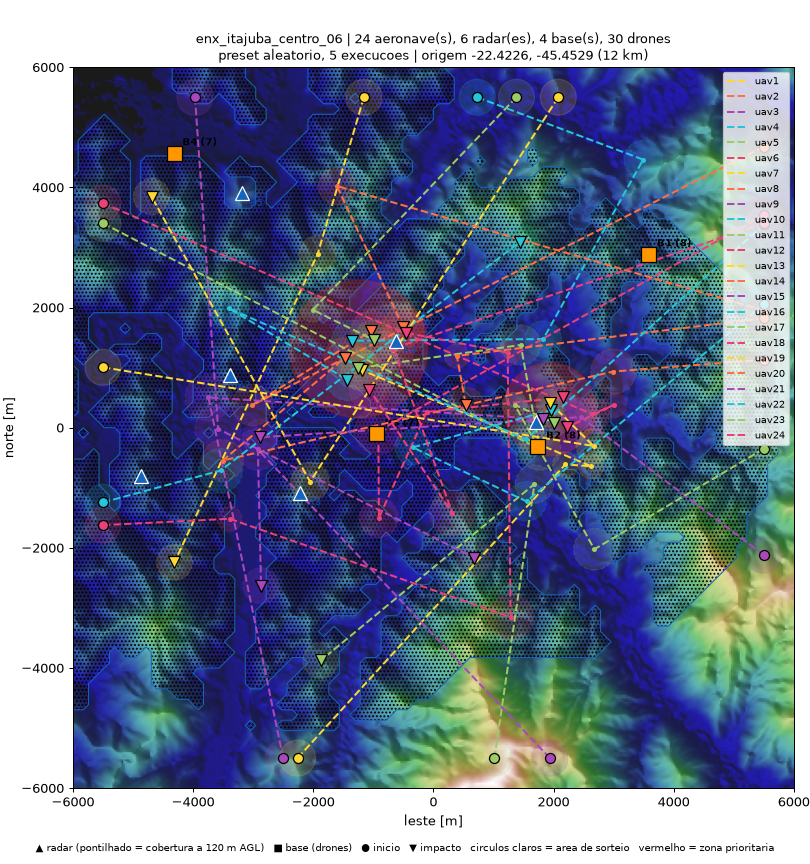
\includegraphics[width=0.7\textwidth]{figs/cenario.png}
\caption{Cenário de teste em Itajubá: 24 aeronaves com perfil misto (rotas tracejadas; $\blacktriangledown$, impactos),
6 radares com a cobertura a 120~m sobre o terreno (pontilhado), 4 bases ($\blacksquare$) e 2 zonas prioritárias
(vermelho).}
\label{fig:cenario}
\end{figure}

% =====================================================================================================
\section{Protocolo experimental}\label{sec:protocolo}
\begin{itemize}
  \item \textbf{Sementes pareadas:} a execução $k$ de cada missão usa a mesma semente para todos os métodos; as
        diferenças entre métodos não vêm de sorteios diferentes.
  \item \textbf{Avaliação:} métodos sem parâmetros aprendidos em todas as 60 missões (300 episódios); métodos aprendidos
        nos 20 cenários de teste, para cada uma das 3 sementes de treino; ablações com 3 execuções por missão.
  \item \textbf{Estatística:} intervalos de confiança de 95\,\% por \emph{bootstrap} reamostrando cenários (episódios do
        mesmo cenário são correlacionados); teste de Wilcoxon pareado contra o húngaro ponderado (M7).
  \item \textbf{Custo:} tempo de decisão medido por chamada, num processador de 8 núcleos, um processo por episódio.
\end{itemize}

% =====================================================================================================
\section{Resultados}\label{sec:resultados}

\subsection{Validação das implementações}\label{sec:validacao}
Em 320 rodadas de decisão de 8 cenários, todos os algoritmos resolveram a mesma instância
(Tabela~\ref{tab:equivalencia}). Os três pares que a teoria diz equivalentes --- leilão e húngaro ponderado (M9, M7), CBAA
e guloso global (M11, M10), MILP e húngaro sobre o WTA (M15, M14) --- atingem o mesmo valor do objetivo em 100\,\% das
rodadas. A designação coincide em 99,6, 100 e 96,8\,\% dos interceptadores; as diferenças vêm de soluções alternativas
com o mesmo valor. Entre os métodos do objetivo~\eqref{eq:F}, o MMR fica em média a 0,1\,\% do melhor valor encontrado,
mas chega a ficar 7,6\,\% abaixo em algumas rodadas; a busca local é a que mais se aproxima (99,99\,\% em média, pior caso
98,6\,\%). O custo varia em duas ordens de grandeza: 4 a 6~ms por rodada para atribuição, leilão, MMR e busca local, 16~ms
para o MILP, 93~ms para o genético, 234~ms para o recozimento e 487~ms para a colônia de formigas.

\inp{tabelas/equivalencia}

\subsection{Escolha da guiagem terminal}\label{sec:res_guiagem}
Antes do benchmark de alocação, um experimento 1$\times$1 (300 encontros por combinação, os mesmos para todas as leis)
comparou leis de guiagem contra cada perfil evasivo (Tabela~\ref{tab:guiagem}), para fixar a lei usada no benchmark e
calibrar $P_T$ em~\eqref{eq:q}. A navegação proporcional com $N'=4$ teve a maior taxa de contato na primeira passagem contra
as manobras não reativas, e sua taxa média de contato na primeira passagem, 0,85, é o valor de $P_T$.
\todo{revisar este parágrafo com o resultado final do experimento.}

\inp{tabelas/guiagem}

\subsection{Comparação dos métodos de alocação}\label{sec:res_alocacao}
\todo{comentar as tabelas principais (teste e treino).}

\inp{tabelas/principal_teste}
\inp{tabelas/principal_treino}

\subsection{Efeito do perfil evasivo e da escala}\label{sec:res_perfil}
\todo{comentar.}

\inp{tabelas/perfil}
\inp{tabelas/tamanho}
\IfFileExists{figs/dano_vs_n.pdf}{\begin{figure}[t]\centering\includegraphics[width=0.7\textwidth]{figs/dano_vs_n.pdf}
\caption{Dano médio nos cenários de teste em função do número de aeronaves.}\label{fig:dano_n}\end{figure}}{}

\subsection{Ablações: troca de alvo, salvas, comunicação e guiagem}\label{sec:res_ablacao}
\todo{comentar.}

\inp{tabelas/ablacao}

\subsection{Métodos aprendidos}\label{sec:res_redes}
\todo{comentar imitação, PPO do zero e refinado, DeepSets $\times$ atenção, variância entre sementes, generalização.}

% =====================================================================================================
\section{Discussão}\label{sec:discussao}
\todo{síntese por família; efeito das manobras evasivas sobre a previsão de velocidade constante; custo e escalabilidade;
recomendações.}

\subsection{Limitações}
\begin{itemize}
  \item \textbf{Modelo de interceptador:} ponto de massa em duas dimensões, com velocidade constante e aceleração lateral
        limitada; sem dinâmica de atitude nem vento.
  \item \textbf{Sensor próprio ideal} na fase terminal.
  \item \textbf{Adaptações:} as técnicas foram adaptadas a interceptadores descartáveis de contato único; M23 perde o
        ramo de reforço, e M15 representa só a parte de alocação de~\cite{cruz2025}, sem obstáculos nem bateria.
  \item \textbf{Modelo de sucesso:} M13--M20 dependem de~\eqref{eq:q}, calibrado num experimento 1$\times$1.
  \item \textbf{Orçamento de treino:} as redes foram treinadas com orçamento fixo e modesto.
\end{itemize}

\section{Conclusão}
\todo{}

\section*{Disponibilidade de código e dados}
O simulador, o gerador de cenários, as 60 missões, as implementações dos 29 métodos e os scripts que geram as tabelas e
figuras estão disponíveis em \todo{repositório}.

\bibliographystyle{unsrtnat}
\bibliography{refs}
\end{document}
